\chapter{Dataset and Preprocessing}

\section{The ROCOv2 dataset}

ROCOv2 {[}7{]} contains 79,789 radiology images (CT, MRI, X-ray, ultrasound, angiography and others) taken from open-access articles on PubMed Central. Each image comes with its figure legend as the caption. We use the official splits (Figure 2.1):

\begin{itemize}
\tightlist
\item
  \textbf{Training set:} updates the weights.
\item
  \textbf{Validation set:} chooses the best epoch.
\item
  \textbf{Test set:} used only once, for the final scores.
\end{itemize}

\begin{figure}
\centering
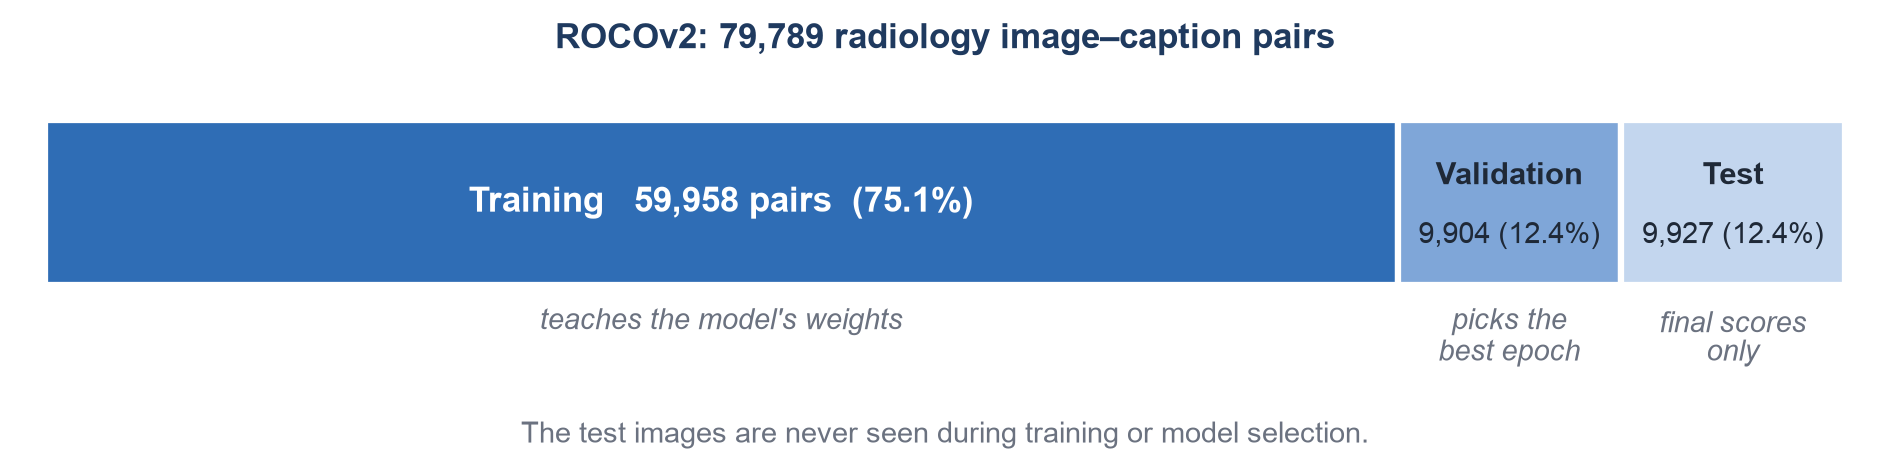
\includegraphics[width=1\linewidth,height=\textheight,keepaspectratio]{figures/fig2_1_splits.png}
\caption{The ROCOv2 splits.}
\end{figure}

The data is very varied, as Figure 2.2 shows. Captions range from 6 words to more than 100, and many refer to marks drawn on the figure, such as ``(*)'' or ``(white arrow)''.

\begin{figure}
\centering
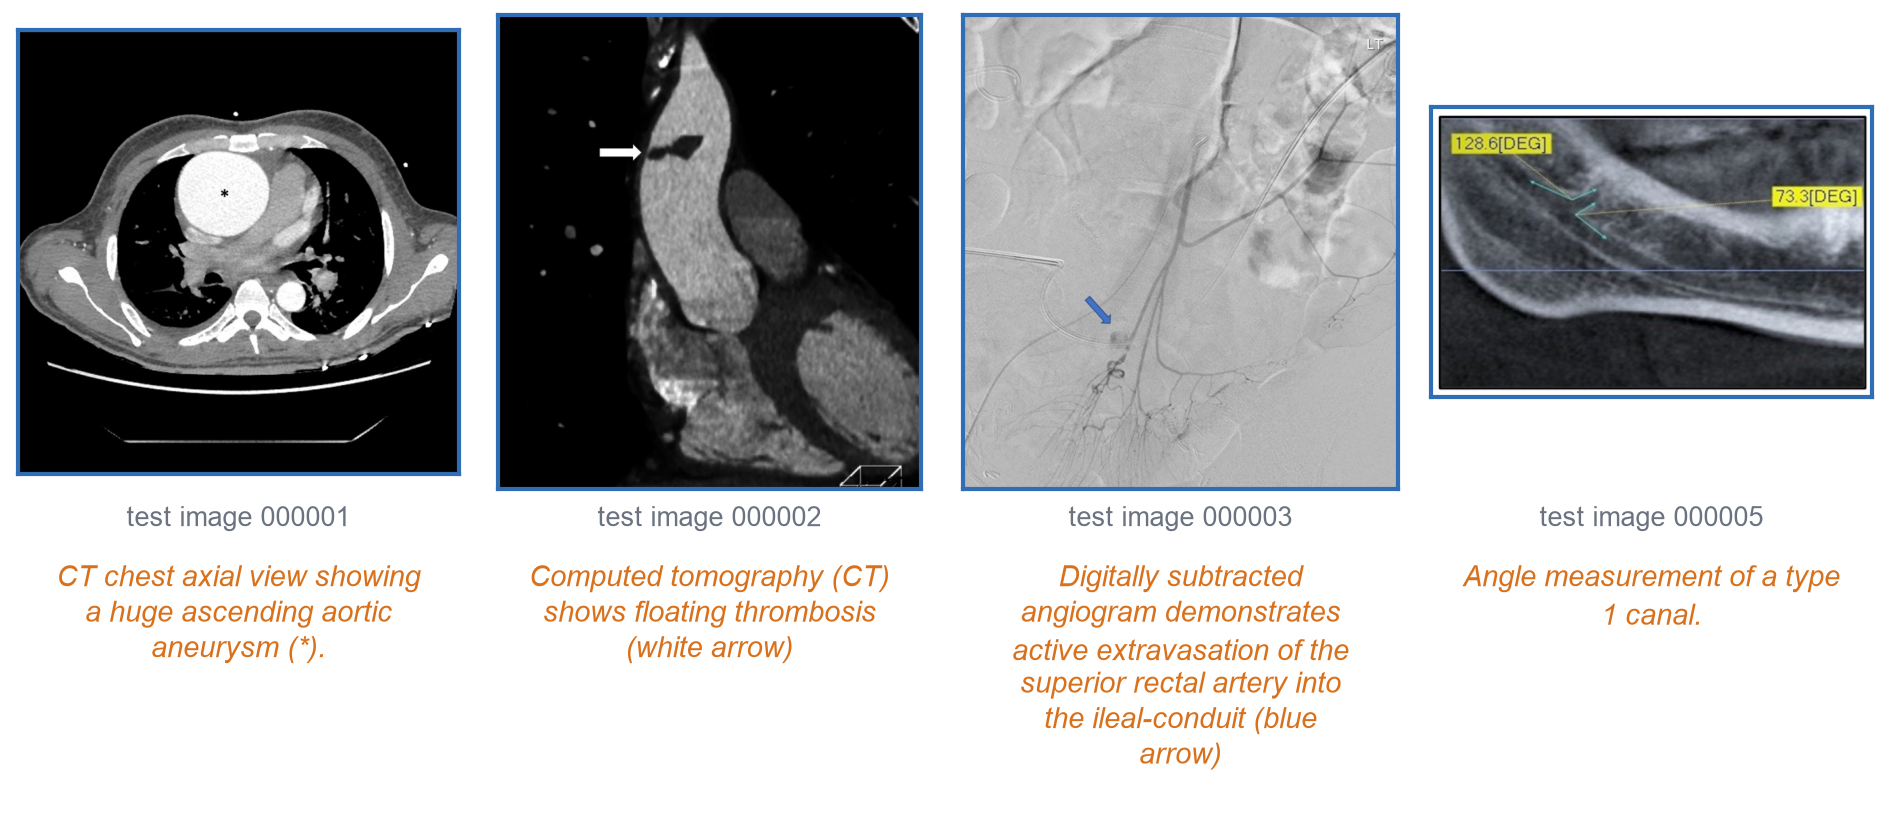
\includegraphics[width=1\linewidth,height=\textheight,keepaspectratio]{figures/fig2_2_samples.png}
\caption{Four ROCOv2 test images with their reference captions.}
\end{figure}

\section{Image preprocessing}

Every scan becomes a \(3 \times 224 \times 224\) tensor (Figure 2.3):

\begin{enumerate}
\def\labelenumi{\arabic{enumi}.}
\tightlist
\item
  \textbf{Resize} to \(224 \times 224\) pixels.
\item
  \textbf{Augment} (training images only): random horizontal flip, rotation of up to \(\pm 10°\), shift of up to 5\%, and brightness or contrast change of up to 10\%.
\item
  \textbf{Normalise} each colour channel with the ImageNet statistics, because the encoder was pretrained on ImageNet {[}10{]}.
\end{enumerate}

Grey scans are copied into all three channels.

\begin{figure}
\centering
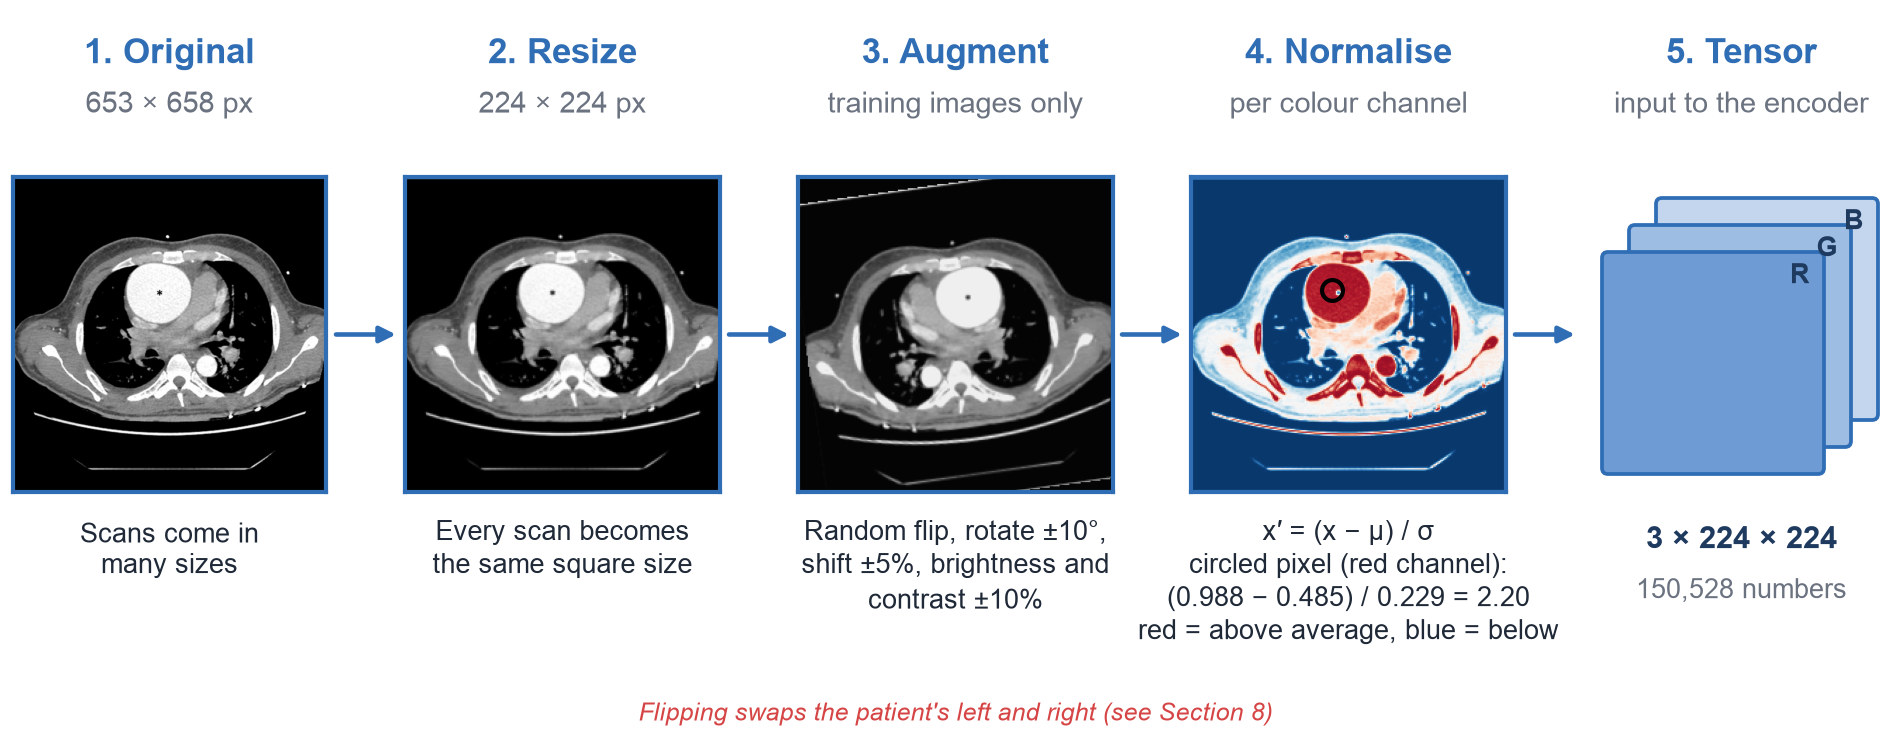
\includegraphics[width=1\linewidth,height=\textheight,keepaspectratio]{figures/fig2_3_preprocess.png}
\caption{The image pipeline on the running example. Augmentation (step 3) is applied only during training.}
\end{figure}

Each pixel value \(p\) (0--255) is first scaled to \(x = p/255\). Then, for each colour channel \(c\):

\[\hat{x}_c = \frac{x_c - \mu_c}{\sigma_c}, \qquad \mu = (0.485,\ 0.456,\ 0.406),\ \ \sigma = (0.229,\ 0.224,\ 0.225) \tag{2.1}\]

\begin{examplebox}

\textbf{Worked example.} The circled pixel inside the aneurysm has \(p = 252\), so \(x = 0.988\). In the red channel this becomes \((0.988 - 0.485)/0.229 = 2.20\). A black background pixel becomes \((0 - 0.485)/0.229 = -2.12\).

\end{examplebox}

\section{Caption preprocessing}

Each caption becomes a list of exactly 40 integers (Figure 2.4), in four steps:

\begin{enumerate}
\def\labelenumi{\arabic{enumi}.}
\tightlist
\item
  \textbf{Clean:} lower-case the text and remove every character that is not a--z or 0--9.
\item
  \textbf{Split:} cut the text into words.
\item
  \textbf{Map to IDs:} replace each word by its position in the \textbf{vocabulary}. The vocabulary holds the 4 special tokens plus every word seen at least 5 times in the training captions: 8,729 tokens in total.
\item
  \textbf{Add start, end and padding:} put \texttt{\textless{}sos\textgreater{}} in front and \texttt{\textless{}eos\textgreater{}} at the end, then pad with \texttt{\textless{}pad\textgreater{}} up to 40 tokens.
\end{enumerate}

The special tokens are \texttt{\textless{}pad\textgreater{}} (ID 0), \texttt{\textless{}sos\textgreater{}} (1), \texttt{\textless{}eos\textgreater{}} (2) and \texttt{\textless{}unk\textgreater{}} (3); any word not in the vocabulary becomes \texttt{\textless{}unk\textgreater{}}.

\begin{figure}
\centering
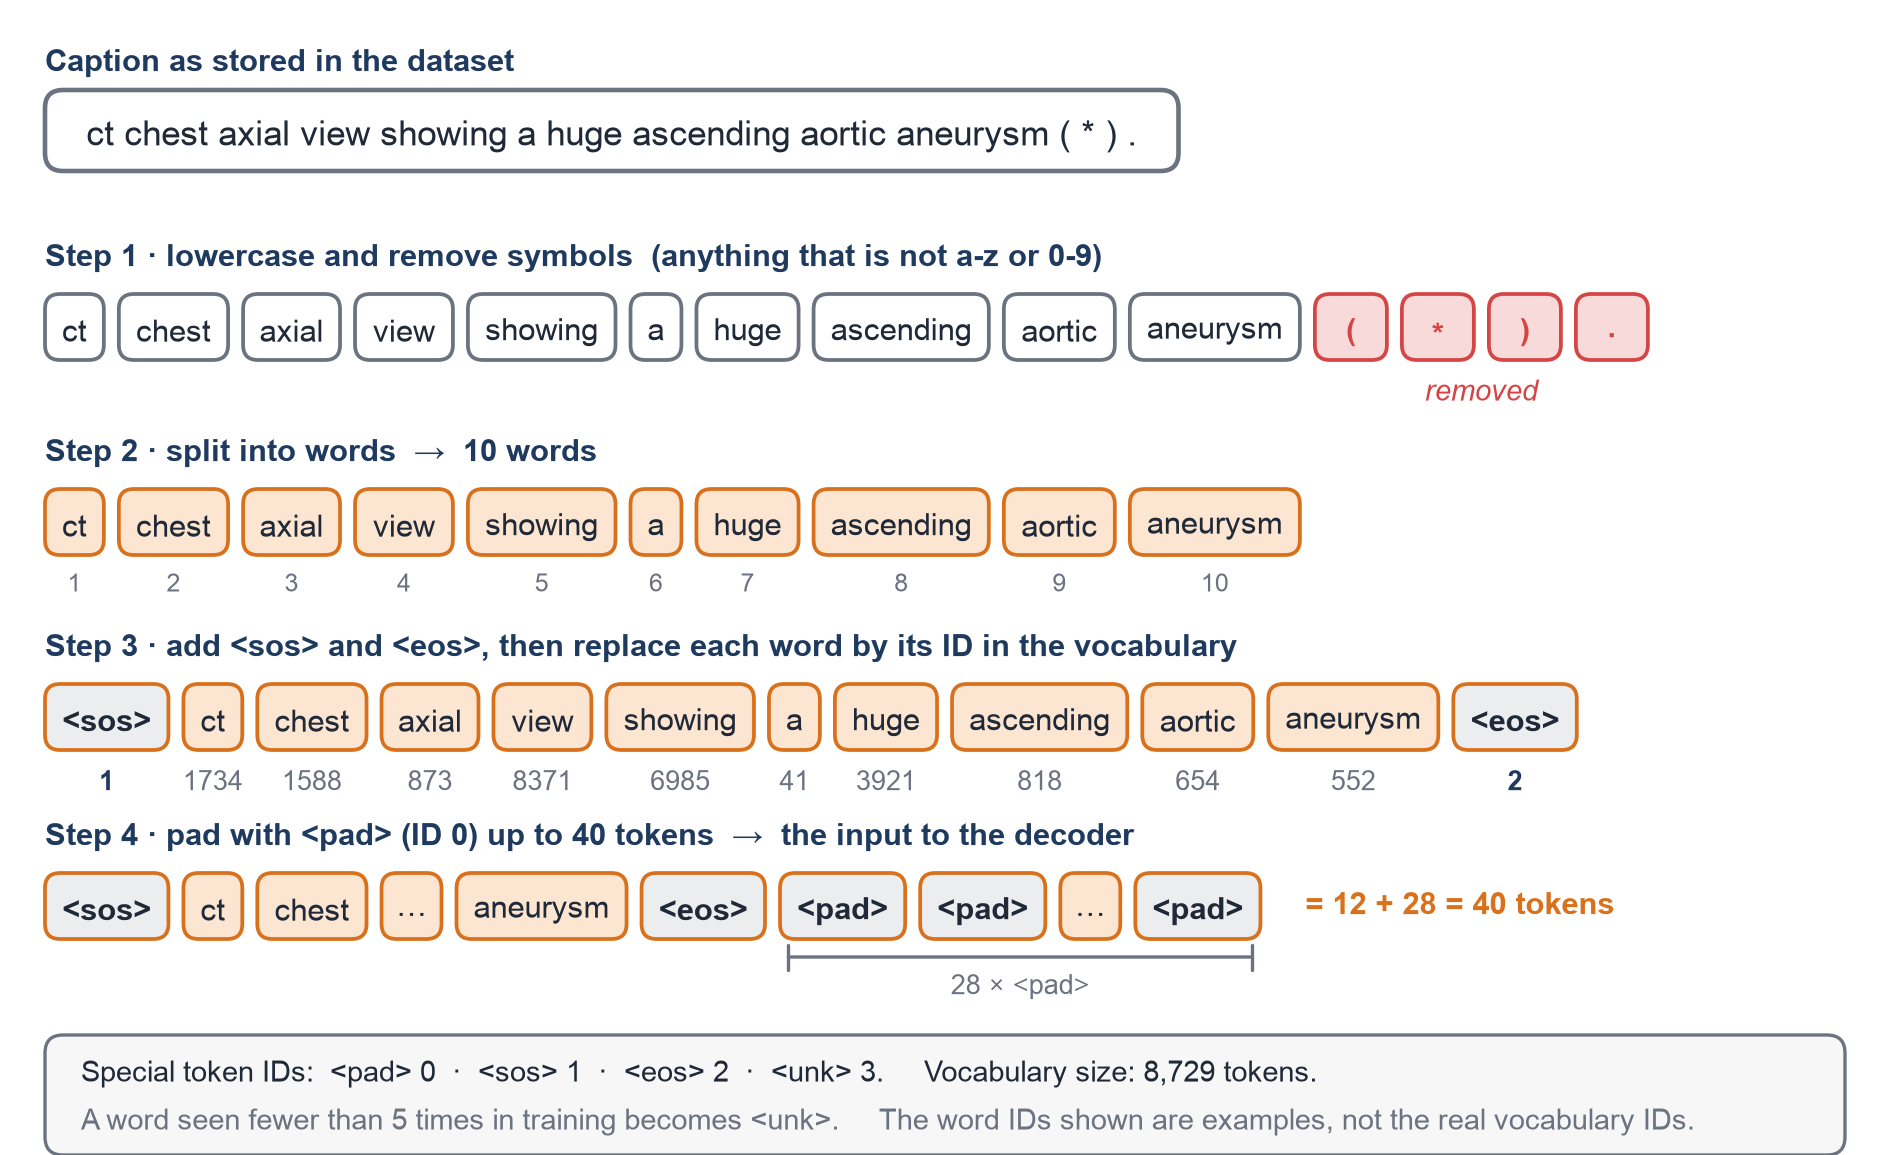
\includegraphics[width=1\linewidth,height=\textheight,keepaspectratio]{figures/fig2_4_tokens.png}
\caption{The caption pipeline on the running example. Ten words plus \protect\texttt{\textless{}sos\textgreater{}} and \protect\texttt{\textless{}eos\textgreater{}} give 12 tokens, followed by 28 padding tokens.}
\end{figure}

With words \(w_1,\allowbreak \ldots,\allowbreak w_n\) and \(T = 40\), the encoded caption is

\[y = \left[\,1,\ \operatorname{id}(w_1),\ \ldots,\ \operatorname{id}(w_m),\ 2,\ 0,\ \ldots,\ 0\,\right], \qquad m = \min(n,\ 38) \tag{2.2}\]

so at most 38 words are kept. One training batch therefore holds an image tensor of shape \((32,\allowbreak 3,\allowbreak 224,\allowbreak 224)\) and a caption tensor of shape \((32,\allowbreak 40)\).
